
\chapter{Methodology}
\label{sec:methodology}


% \subsection{?implementational details of testing software? (pos, bash, moongen lua)}


% Analyzes and assesses several possible approaches that solve the problem

% why used testing methods: latency, throughput, perf/cache-misses

In this paper the performance of \Ac{vpp} is quantified by throughput
and latency which can be measured by the MoonGen
\cite{emmerich2015moongen} load generator. To help identifying
bottlenecks and limiting factors, \Ac{perf} is used to measure metrics
like cache misses and clock cycle counts. Furthermore \Ac{vpp}'s error
counters are collected after each run, to detect problems in the
packet processing tests.


\section{Measurement Results}

% methods of metric retrieval

% moongen 

\subsection{MoonGen (Throughput and Latency)} 

% TODO talk about threading

The \Ac{dut} sends test traffic using Moongen. There is a lua script
determining MoonGen's behaviour for generating layer 2 ethernet
packets, another one for layer 3 \Ac{ip4} packets, one for \Ac{ip6}
packets and one for \Ac{vxlan} packets. All but the latter can be
given command line parameters to cap the packet rate, change the
packet size, the destinations, the sources and the amount of
destinations to send to.

Additionally the scripts grant \Ac{vpp} some warmup time: Only when
the first packet is successfully forwarded, the actual test begins.
This is necessary, because \Ac{vpp} v18.10 tends to drop packets in
the interface-tx node for a few seconds when it is not warmed up which
could drasically distort the average throughput and latency. After the
other components have settled into the high load situation which takes
around a second, the throughput average stays about constant and can
thus be properly described by the average and standard deviation.

To measure the latency, occasional, timestamped packets are sent by
MoonGen between the load generating packets. This is used to calculate
average and standard deviation and create a histogram of latencies.


\subsection{\Ac{perf}}

\paragraph{perf-stat} 

The command \lstinline|perf stat| is used to attatch to the
\lstinline|vpp_main| process. This allows collection of hardware
counter information about different types of cache events, cpu cycles
used etc. The stats of all children are added up to the main thread's
ones.

\paragraph{perf-record/perf-report}
\label{sec:perf}

The command \lstinline|perf record| is used to attatch to the first
worker thread of \Ac{vpp} or if vpp runs singlethreaded, to the main
thread. This records the cpu time spent per function (symbol). It is
important to connect to a thread processing the packet in \Ac{vpp}'s
graph (not necessarily the main process) to get significant results
for identifying performance limiting factors. After the test run, the
record has to be parsed with \lstinline|perf report| to associate
function names to the symbols.

\paragraph{Performance Impact}

Those two tools run during the test and can therefore impact the
\Ac{dut}'s performance. For \Ac{ip4} forwarding the impact can be up
to 8\% decrease from the original packet throughput rate. That's why
the \Ac{perf} tools are only active for graphs showing cache misses or
time spent per function. 


\subsection{\Ac{vpp} Counters: socat}
\label{sec:vppcounters}

Additionally \Ac{vpp} internal counters, usually used for error
counting, are saved into the test's report for test quality assurance
and debugging. The counters can be read via the \lstinline|show
errors|  \Ac{cli} command. Therefore \Ac{vpp} is configured to listen
at a unix file fifo for it's \Ac{cli}. This interface can be
conveniently used with the tool "vppctl" in \Ac{vpp} v18.10 to connect
and interact with the fifo. In earlier versions like v16.09 this tool
worked differently. In order to be able to read those counters
nevertheless, the tool "socat" was used to connect to the \Ac{cli}
fifo file.


\section{Test Procedure}

One test run tests one \Ac{vpp} configuration. After each test run,
\Ac{vpp} is beeing restarted. After each restart, the performance of
\Ac{vpp} varies significantly more than within one testrun. Therefore
in order to get an insight in how spread the variance is, each test
run is repeated 6 times. Only histogram latency measurements rely on a
single run.

As figure \ref{testsequence} shows, the \Ac{dut} and \Ac{loadgen}
first read the remote configuration file, after the management server
has started the test. Afterwards both devices configure the Intel
pstate driver  as described in section \ref{sec:hardware} and the
\Ac{dut} loads the kernel module for the NIC's. Then \Ac{dut} and
\Ac{loadgen} are synchronized as the pre-test \textit{setup is
complete}.

Before starting the new \Ac{vpp} daemon, the old one is killed and
some files which may contain global state are removed. The \Ac{vpp}
daemon will take at most a few seconds to set itself up, so both
devices are synchronized again and MoonGen is already beeing started,
because it's setup takes longer. When MoonGen is set up and starts
it's warmup loadgen-phase, \Ac{vpp} is already online. \textit{20
seconds} after MoonGen started, both systems are \textit{running and
have stabilized}.

Now, after both systems synchronized again, \textit{\Ac{perf} data is
collected} as described in section \ref{sec:perf} for a timespan of 10
seconds. Then both systems synchronize again, \Ac{vpp}'s counters are
queried (section \ref{sec:vppcounters}), MoonGen is killed and after
giving it 10 seconds time to finalize the throughput and latency
histogram, all files containing test results are uploaded to the
management server.

Approximately 43 seconds after the test started, the final
synchronization takes place an the \textit{next run can be started}.

\begin{figure}[!ht]
\noindent\hspace{0.5mm}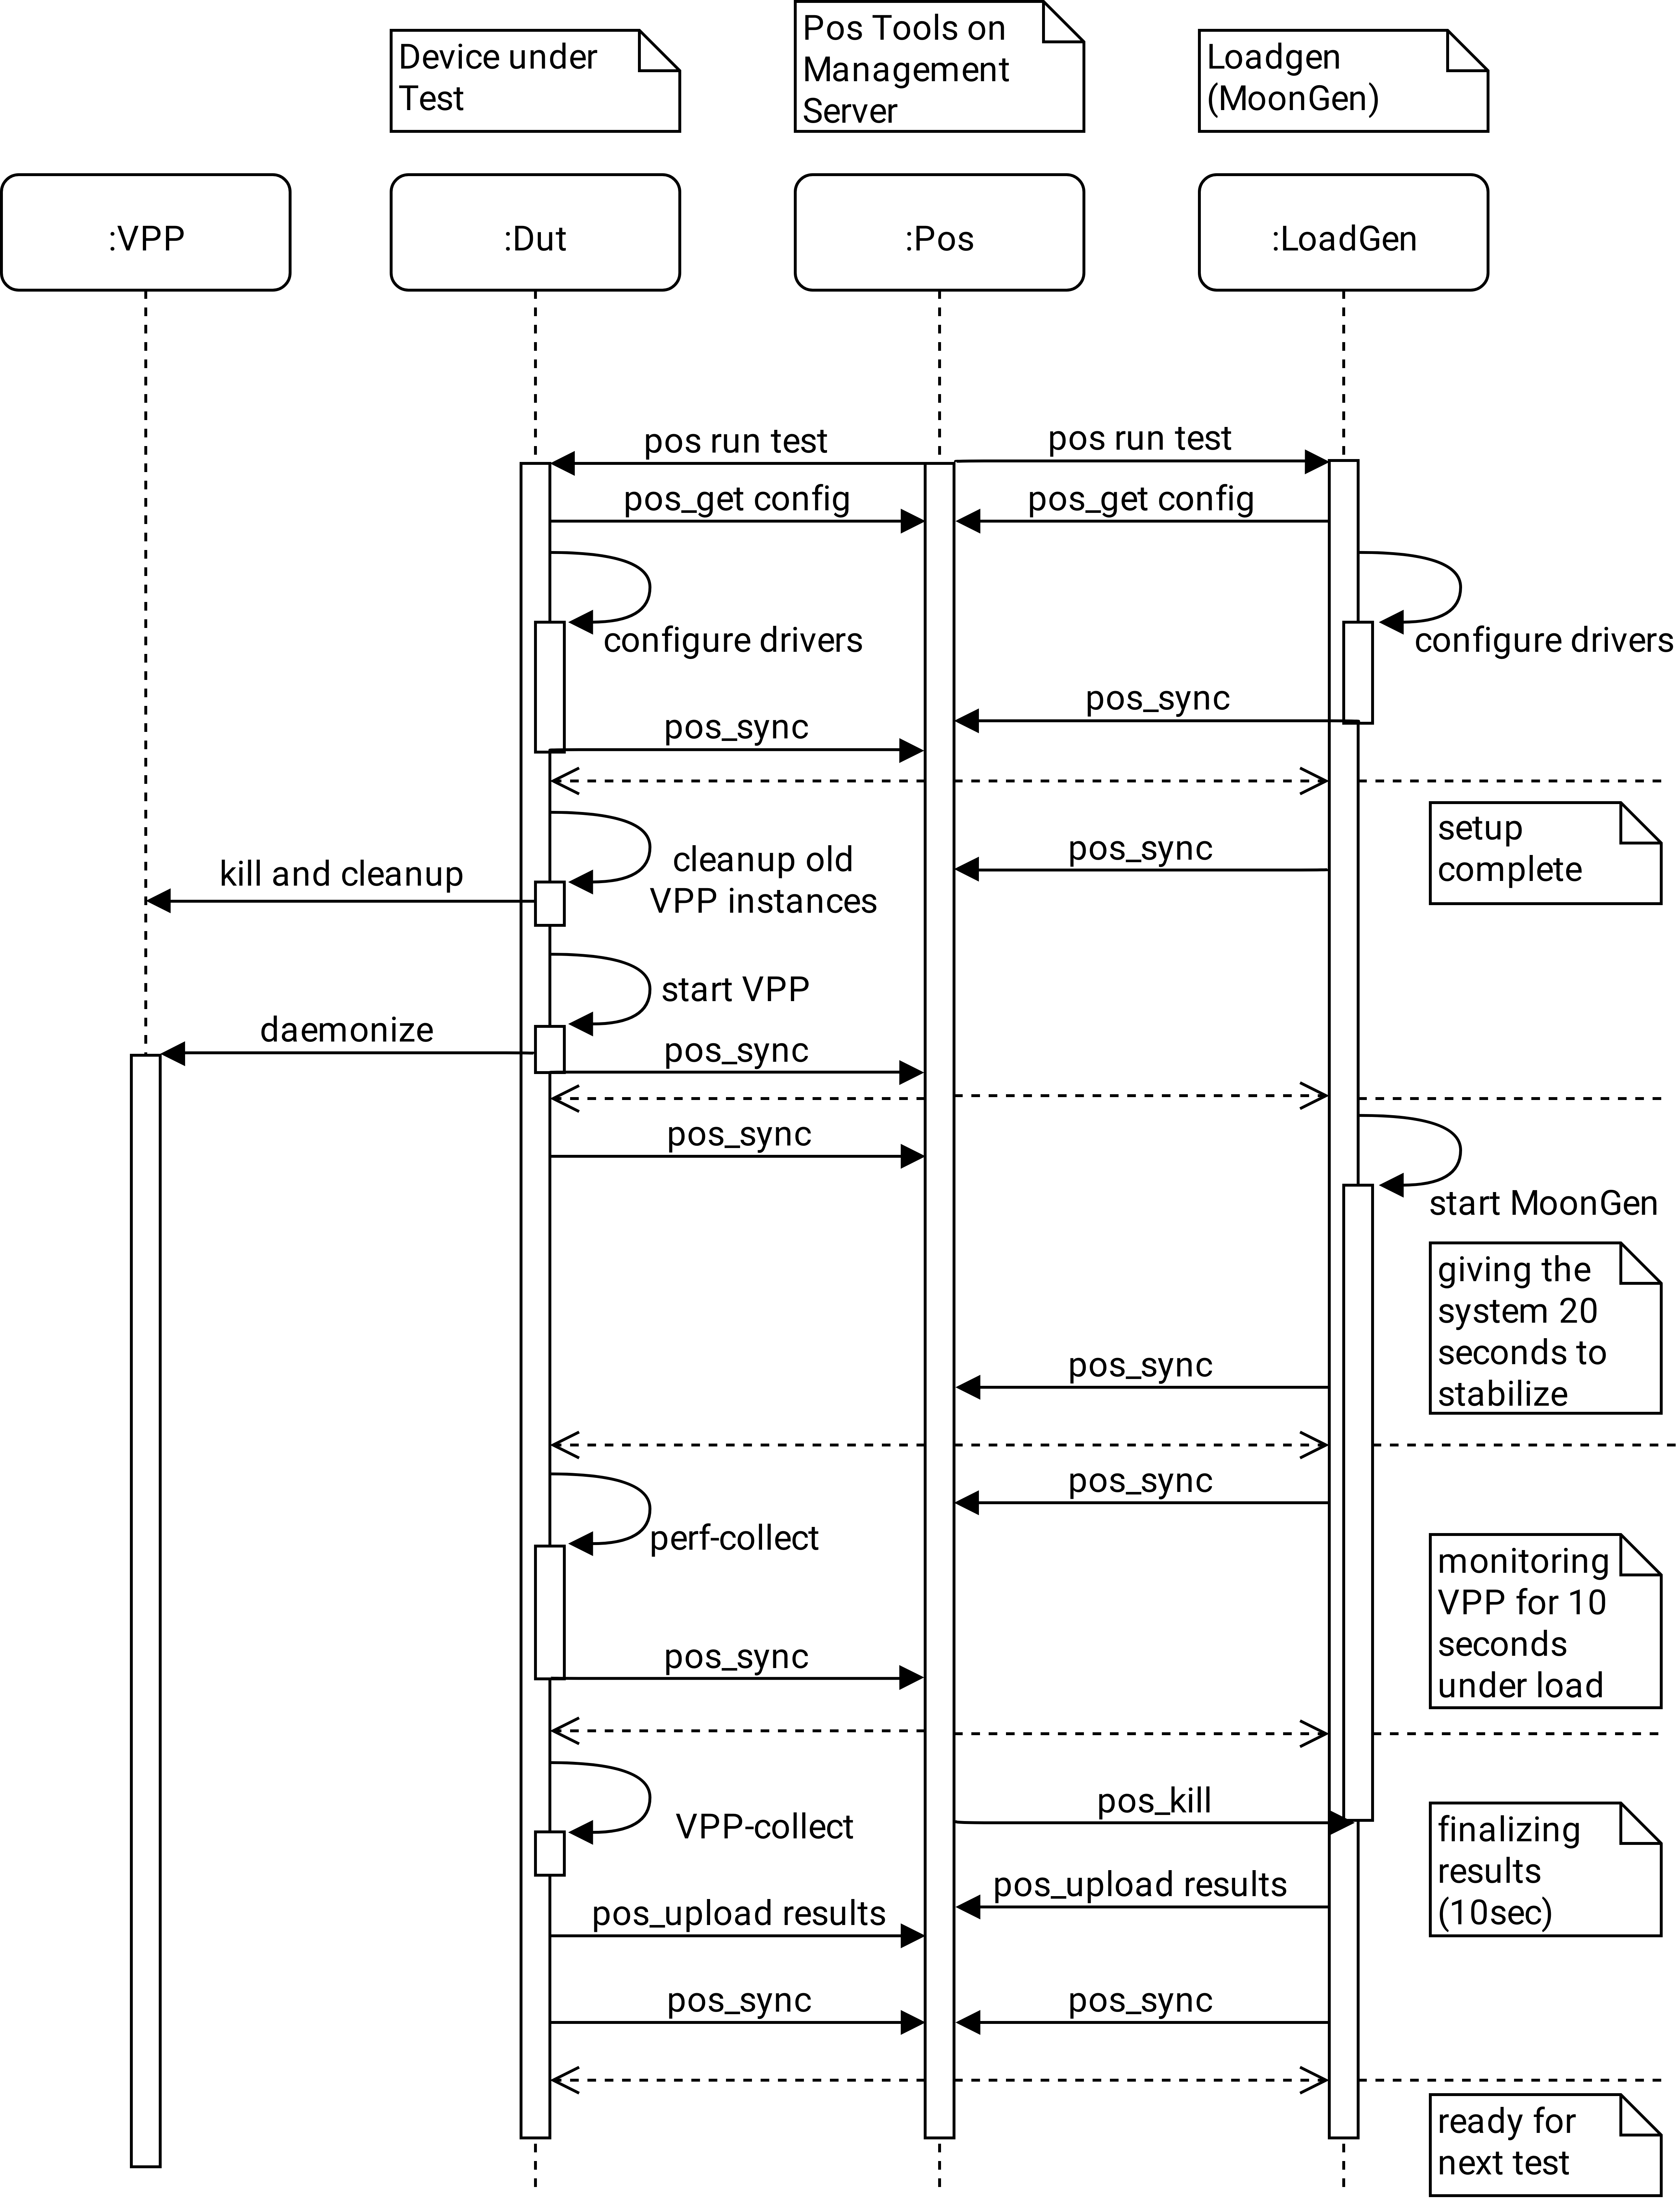
\includegraphics[width=\linewidth]{pics/procedure-sequence.png}
\caption{Sequence of a single testrun. }
\label{testsequence}
\end{figure}


\section{Configuring \Ac{vpp}}

% describe/explain vpp configs/execs

Configuring \Ac{vpp} consists of two steps: Setting the startup
parameters which is done using a \Ac{config} - and executing \Ac{cli}
commands to configure the routing settings on runtime. For the latter
a file containing the \Ac{cli} commands can be specified in the
startup \Ac{config} to be executed. 

The \Ac{vpp} starting scripts used for this paper therefore create
temporary \Ac{config} and \Ac{exec} for example according to the
number of \Ac{ip4} routes specified in the starting script's
parameters. The \Ac{ip4} and \Ac{ip6} scripts also support arbitrary
multicore (-pinning) configurations.

% for the l2fib size tests a plugin was written to add cli support for adding multiple entries with one command.  

Adding millions of \Ac{ip4} or \Ac{ip6} entries to the layer 3
\Ac{fib} is no problem, because the \Ac{cli} already has a command
parameter to add any number of entries through a single command. The
\Ac{cli} commands for the layer 2 \Ac{fib} don't support this though.
Adding millions of entries via the command line would be too time
consuming. That's why this paper uses an own \Ac{vpp} plugin which
extends the \Ac{cli} by a command with this functionality. In terms of
speed it is comparable with the built-in commands.


\section{Tested Scenarios}

For this paper there are many \Ac{vpp} configurations to test several
scenarios:

\paragraph{XConnect} 

The most simple configuration is linking two network interfaces via
cross connect (xconnect). This is a static mapping from one
interface's input to another interface's output and vice versa.

\paragraph{L2 bridging}

For layer 2 switching \Ac{vpp} can create bridge domains. The optional
bridge features mac-learning and mac-aging impact performance when
activated, even when not specifially tested. Other features like
flooding settings have no significant performance impact when not
directly tested. Therefore in section \ref{sec:cpubottleneck} results
are presented with and without the impacting features enabled.

\paragraph{L3 routing}

The \Ac{ip4} and \Ac{ip6} routing tests use multiple routes which all
point to the same destination, conforming RFC2544.

\paragraph{\Ac{vxlan}}

Setting \Ac{vpp} up to encapsulate \Ac{vxlan} packets takes amongh
others the following steps:

\begin{enumerate}
	\item Add a dedicated IP \Ac{fib} table and configure it to route to the \Ac{vxlan} decapsulation endpoint.
	\item Create a bridge domain belonging to the dedicated IP table.
	\item Setup the tunnel using the bridge domain and the dedicated IP table.
	\item Add the new virtual \lstinline|vxlan-tunnel*| interface and all other necessary interfaces to the bridge domain and take care of all of their l2fib entries. 
\end{enumerate}

This means all packets arrive in the bridge domain, are forwarded to
the virtual vxlan-tunnel interface, then encapsulated and sent to the
vxlan-tunnel endpoint via IP.


\section{Testbed Hardware Setup}
\label{sec:hardware}

Test are conducted on different test systems listed in table
\ref{table:hardware}. All of the used systems (the \Ac{loadgen} ones,
too) are configured via the Intel Pstate driver to disable turbo boost
in order to maintain a close to constanct clock speed.

% lscpu
% lshw -C memory
% apt install i2c-tools
% modprobe eeprom
% decode-dimms

\begin{table}[!ht]
	
	\vspace{3ex}
	\begin{tabular}[]{ l | c | c | c }
		DUT & NIC Model & NIC type & RAM \\ \hline
		klaipeda & Intel 82599 & 2x10GbE & DDR3 1333 MHz CL9-9-9-24 \\
		omastar & Intel XL710 & 2x40GbE & DDR4 2133 MHz CL15-15-15-35
	\end{tabular}

	% TODO check this for neccessarity and correctness
	\vspace{2ex}
	\begin{tabular}[]{ l | c | r | r | r | r }
		DUT & CPU @ clock (GHz) & pyhsical cores & L1 cache & L2 cache & L3 cache \\ \hline
		klaipeda & Xeon E3-1230 @ 1.6-3.2 & 4 & 32k & 256k & 8M \\ % 2^23
		omastar & Xeon E5-2630 v4 @ 1.2-2.2 & 10 & 32k & 256k & 25M % 2^
	\end{tabular}

	\caption{\Ac{dut} hardware: CPU model with minimum and maximum clock speed reachable with the Intel Pstate driver without turbo boost, \Ac{nic} model and \Ac{ram} timings}
	\label{table:hardware}
\end{table}

% {details about testbed setup (used servers and configs)}

% cpu config, driver config

% exact test setup description

